\documentclass[12pt]{article}
\usepackage[utf8]{inputenc}
\usepackage{graphicx}
\usepackage{amsmath}
\usepackage{geometry}
\usepackage{booktabs}
\usepackage{float}
\usepackage{pdfpages}
\usepackage{rotating}
\geometry{a4paper, margin=1in}


\begin{document}
\section*{Task 1: CMOS Inverter Simulation}
The circuit diagram for Task 1 is shown in Figure \ref{fig:task1}. The circuit includes an output load capacitor, whose value is systematically varied (1\,\textmu F, 2.2\,\textmu F, and 220\,\textmu F) to observe its effect on the inverter's transient response.

\begin{figure}[H]
    \centering
    
\includegraphics[width=0.75\textwidth]{images/task1_circuit.png}
    \caption{Task 1 - CMOS Inverter Circuit Diagram}
    \label{fig:task1}
\end{figure}

\subsection*{Task 1.1: C = 1\,\textmu F}
When the output load capacitor is set to 1\,\textmu F, the transient response of the inverter is observed.
\begin{figure}[H]
    \centering
    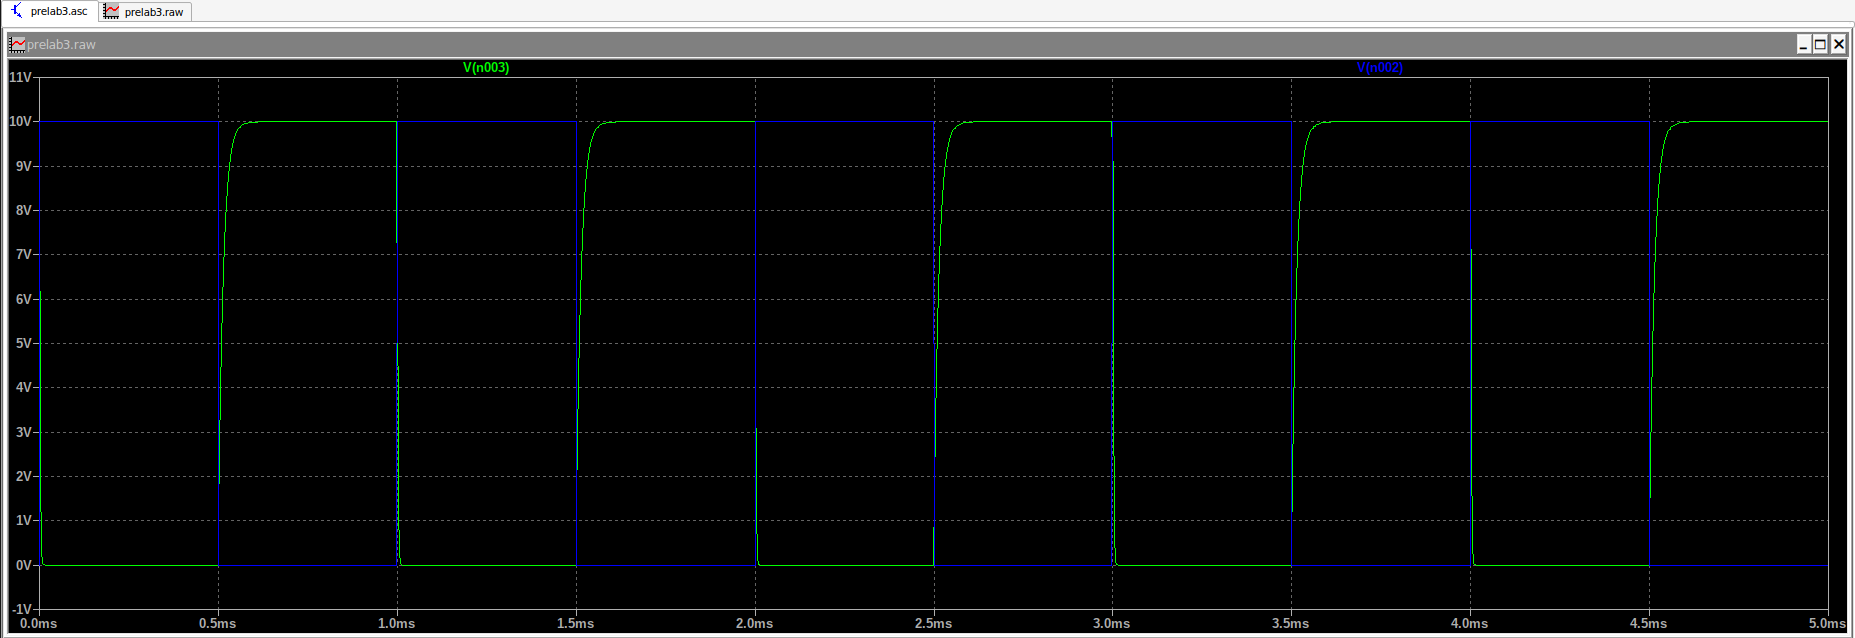
\includegraphics[width=1\textwidth]{images/task1_1uF.png}
    \caption{Transient Response with C = 1\,\textmu F}
    \label{fig:task1_1uF}
\end{figure}

\newpage

\subsection*{Task 1.2: C = 2.2\,\textmu F}
When the output load capacitor is increased to 2.2\,\textmu F, thetransient response of the inverter is observed again.
\begin{figure}[H]
    \centering
    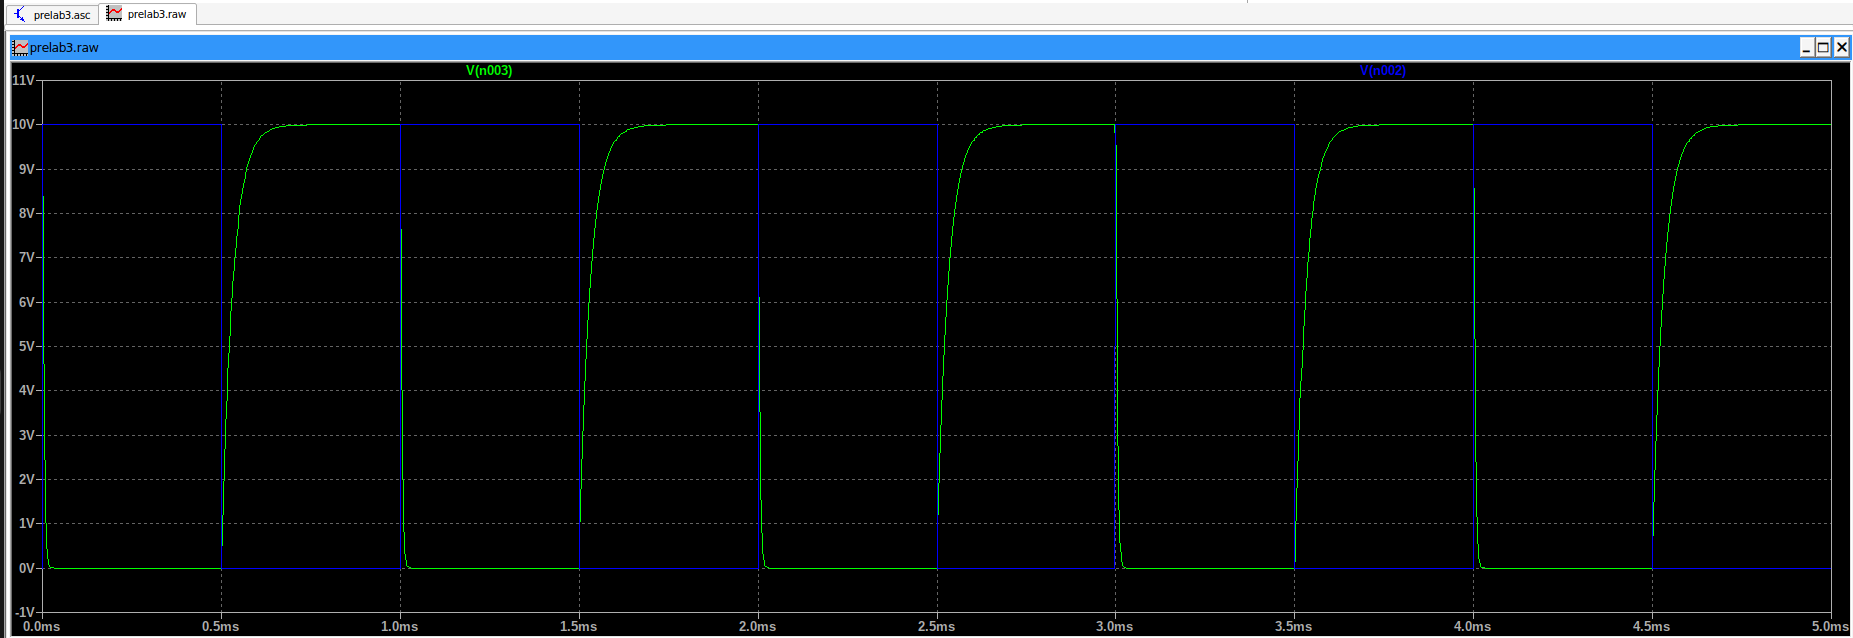
\includegraphics[width=1\textwidth]{images/task1_2_2uF.png}
    \caption{Transient Response with C = 2.2\,\textmu F}
    \label{fig:task1_2_2uF}
\end{figure}

\subsection*{Task 1.3: C = 220\,\textmu F}
When the output load capacitor is drastically increased to 220\,\textmu F, the transient response of the inverter is severely degraded, as illustrated in Figure \ref{fig:task1_220uF}. Unlike the previous tasks, the output completely fails to reach a full voltage swing (0\,V to 10\,V) within the 1\,ms period. Because the RC time constant is now significantly larger than the 0.5\,ms input pulse width, the capacitor cannot fully charge or discharge, resulting in a heavily attenuated, asymmetrical waveform.

\begin{figure}[H]
    \centering
    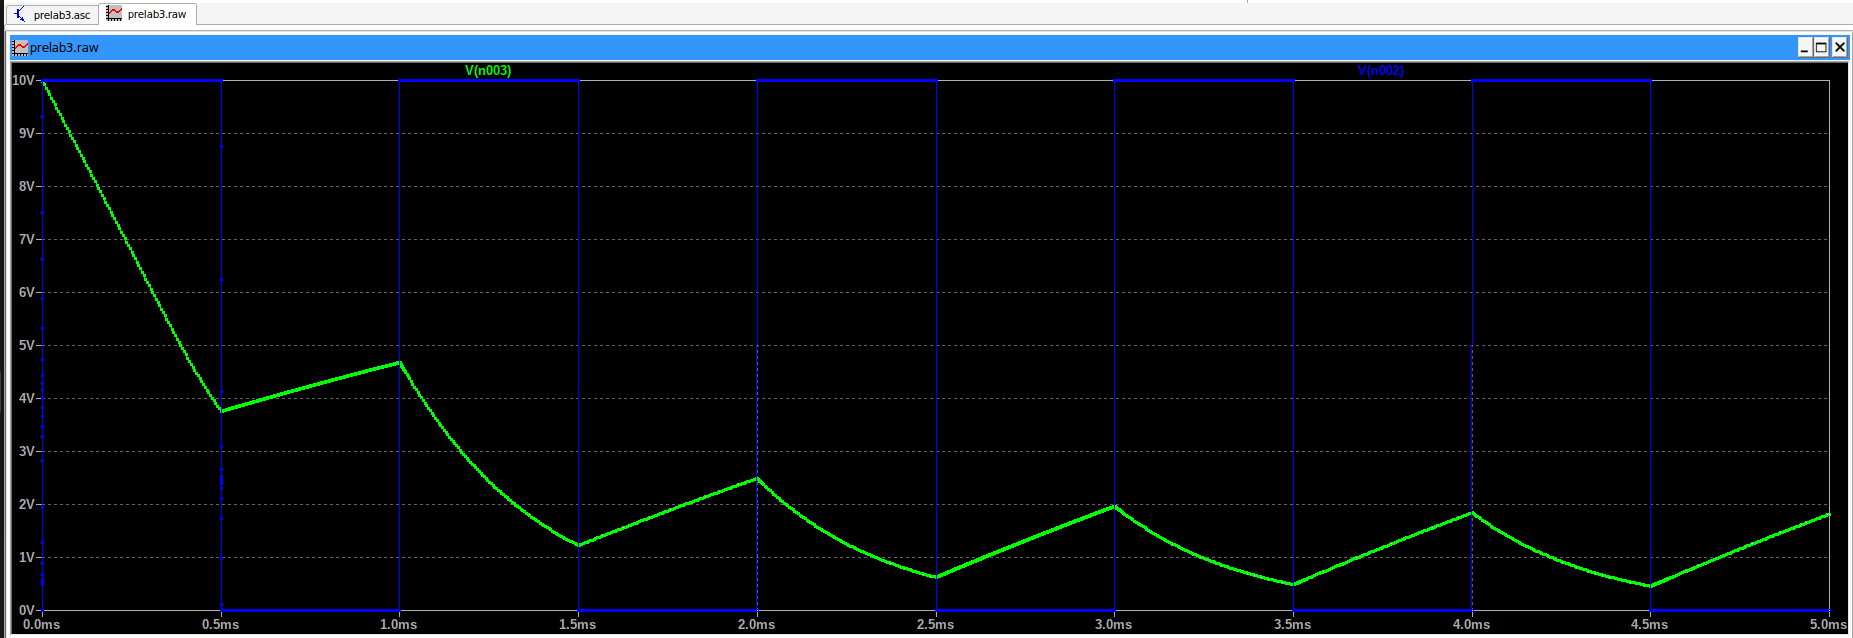
\includegraphics[width=1\textwidth]{images/task1_220uF.png}
    \caption{Transient Response with C = 220\,\textmu F}
    \label{fig:task1_220uF}
\end{figure}

\subsection*{Analysis}

\textbf{Effect of Capacitance on Switching Speed:} \\
Increasing load capacitance decreases switching speed. The transition time is dictated by the time constant $\tau = R_{ds(on)} \cdot C_{load}$. While the 1\,\textmu F load switches almost instantly, the 220\,\textmu F load creates a $\tau$ too large for the 1\,kHz frequency, proving that large capacitive loads severely limit maximum operating speed.

\vspace{0.3cm}

\textbf{Analysis of Rise and Fall Times:} \\
The rise and fall times are asymmetrical due to differing PMOS and NMOS characteristics:
\begin{itemize}
    \item \textbf{Fall Time ($t_f$):} Faster. The NMOS (2N7000) utilizes higher-mobility electrons, resulting in a low on-resistance ($R_n \approx 5\,\Omega$) and rapid discharge to ground.
    \item \textbf{Rise Time ($t_r$):} Slower. The PMOS (ZVP3306A) relies on lower-mobility holes, resulting in a higher on-resistance ($R_p > R_n$) and a slower charge to 10\,V.
\end{itemize}

\section*{Task 2: Ring Oscillator Simulation}

The 3-stage ring oscillator circuit is shown in Figure \ref{fig:task2_circuit}. 

\begin{figure}[H]
    \centering
    
\includegraphics[width=0.8\textwidth]{images/task2_circuit.png}
    \caption{Task 2.1 - 3-Stage Ring Oscillator Schematic}
    \label{fig:task2_circuit}
\end{figure}

To accurately extract the oscillation parameters without relying on manual cursors, the following \texttt{.meas} directives were executed in LTspice:

\begin{verbatim}
.meas tran V_Max MAX V(Vin)
.meas tran V_Min MIN V(Vin)
.meas tran V_Mean AVG V(Vin)
.meas tran Period_T TRIG V(Vin) VAL=2.5 RISE=5 TARG V(Vin) VAL=2.5 RISE=6
.meas tran Frequency PARAM 1/Period_T
\end{verbatim}

The automated results extracted from the SPICE Error Log are tabulated below.

\begin{table}[H]
    \centering
    \begin{tabular}{|l|c|}
        \hline
        \textbf{Parameter} & \textbf{Measured Value} \\ \hline
        Maximum Voltage ($V_{max}$) & 5.02\,V \\ \hline
        Minimum Voltage ($V_{min}$) & -0.03\,V \\ \hline
        Mean Voltage ($V_{mean}$) & 2.28\,V \\ \hline
        Oscillation Period ($T$) & 88.01\,ns \\ \hline
        Oscillation Frequency ($f$) & 11.36\,MHz \\ \hline
    \end{tabular}
    \caption{Transient Measurement Results}
    \label{tab:osc_results}
\end{table}

\begin{figure}[H]
    \centering
    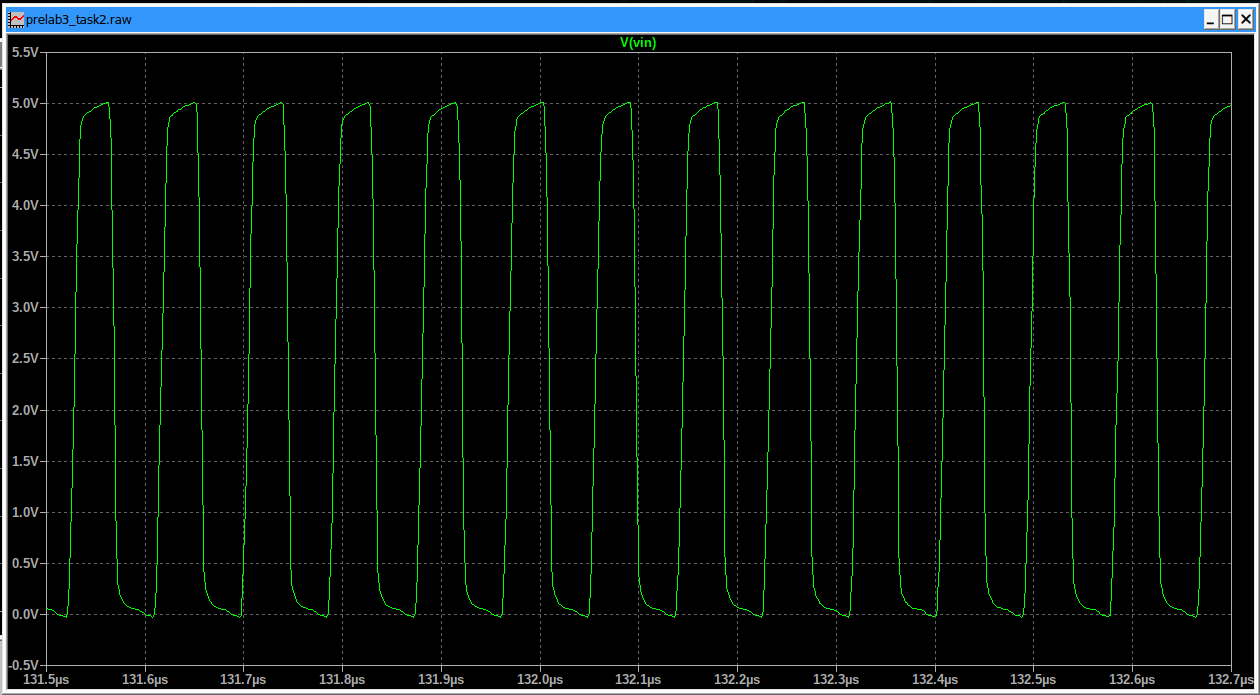
\includegraphics[width=1\textwidth]{images/task2_plot.png}
    \caption{Transient Response of the 3-Stage Ring Oscillator}
    \label{fig:task2_transient}
\end{figure}

\vspace{0.3cm}
\textbf{FFT Analysis and Reflection:} \\
An FFT analysis was performed on the output waveform to observe its frequency spectrum. As shown in Figure \ref{fig:task2_fft}, manual inspection confirms that the fundamental frequency peak occurs exactly at 11.36\,MHz, which perfectly aligns with our transient period calculations. Finally, the measured mean voltage of 2.28\,V (rather than a perfect 2.5\,V) highlights a slight drive asymmetry, indicating the NMOS device pulls the node to ground slightly faster than the PMOS pulls it to the 5\,V rail.

\textit{(Note: To preserve the detail of the frequency spikes, the FFT spectrum in Figure \ref{fig:task2_fft} is presented in a landscape orientation on the new page for enhanced readability.)}

\clearpage % Forces everything above to print, then starts a new page

\begin{sidewaysfigure}
    \centering
    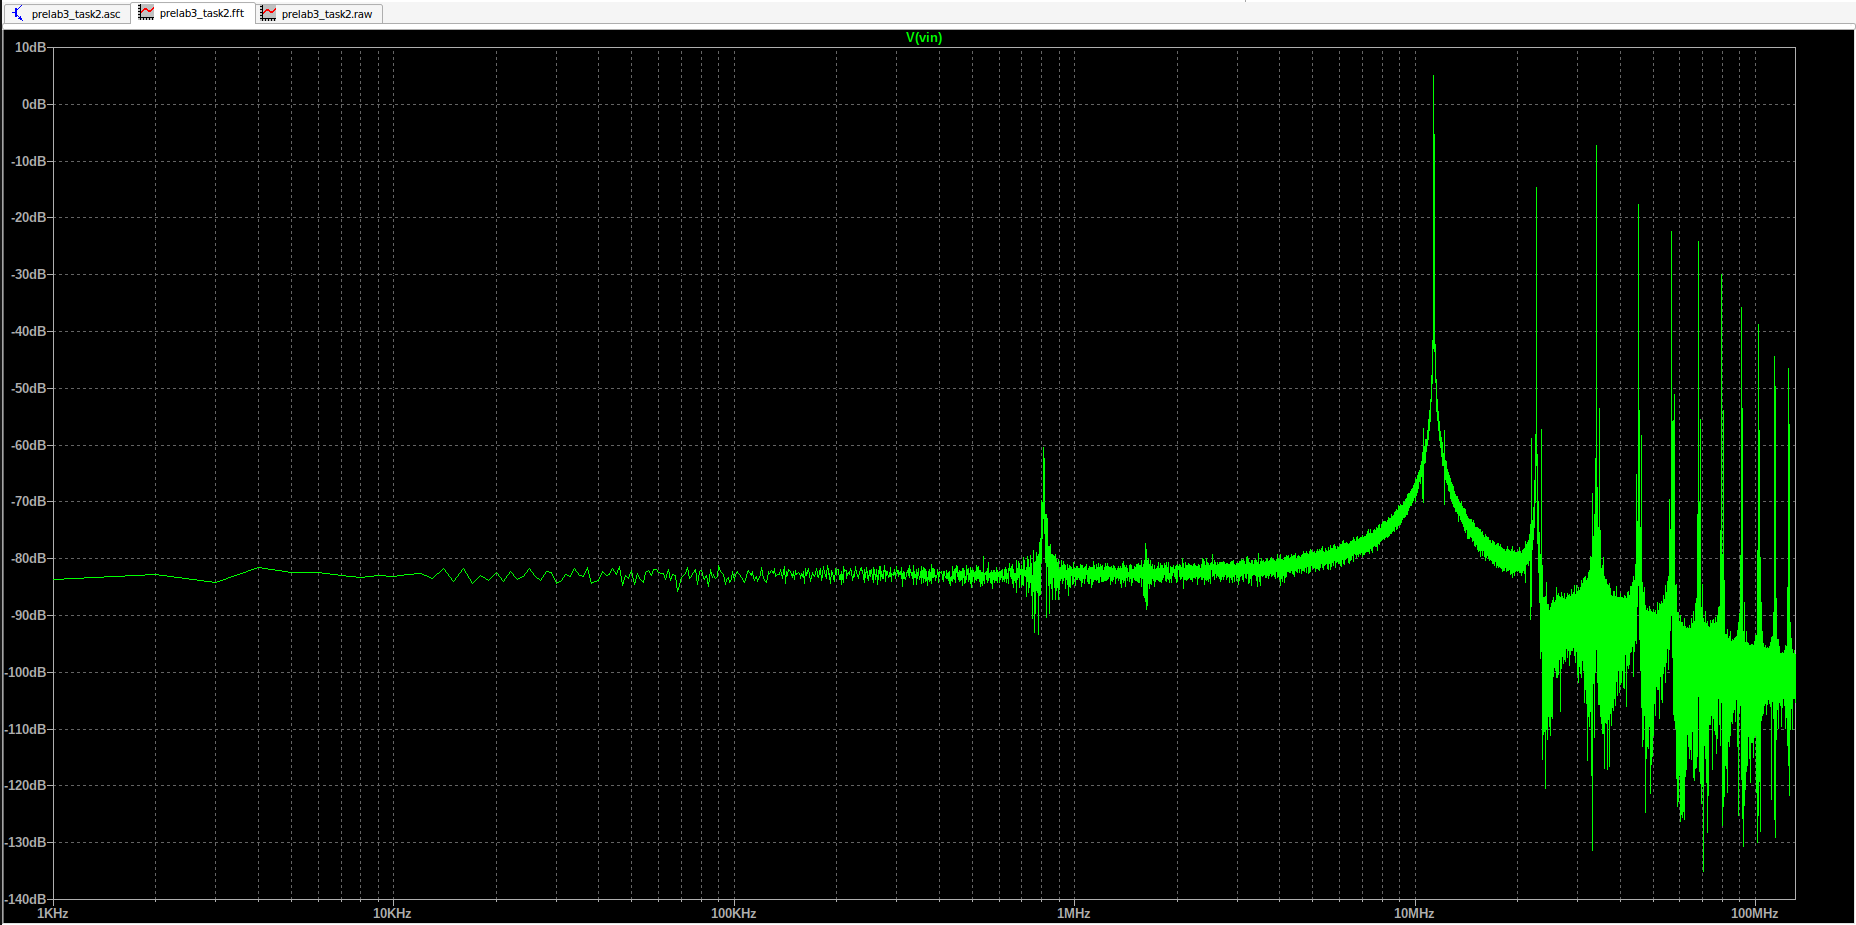
\includegraphics[width=\linewidth]{images/task2_fft.png}
    \caption{FFT Spectrum demonstrating the fundamental frequency and odd harmonics.}
    \label{fig:task2_fft}
\end{sidewaysfigure}

\clearpage % Ensures the next section starts on a normal portrait page
\end{document}